\documentclass[11pt]{article}

\usepackage[margin=1in]{geometry}
\usepackage{amsmath, amssymb}
\usepackage{booktabs}
\usepackage{graphicx}
\usepackage{float}
\usepackage{hyperref}
\usepackage{xcolor}
\usepackage{enumitem}
\usepackage{subcaption}

\hypersetup{
    colorlinks=true,
    linkcolor=blue,
    urlcolor=blue,
    citecolor=blue
}

\newcommand{\TODO}[1]{\textcolor{red}{\textbf{TODO:} #1}}
\newcommand{\class}[1]{\texttt{#1}}

\title{EE/CS 148B Homework 3: Vision-Language Models}
\author{Aditya}
\date{\today}

\begin{document}

\maketitle

\section{Vision Transformer}

\subsection{Patch Embeddings}

\TODO{Briefly state that \class{PatchEmbeddings} was implemented in \class{basics/vit.py}. No written response is required unless you want to mention any implementation detail.}

\subsection{ViT}

\TODO{Briefly state that \class{ViT} was implemented in \class{basics/vit.py}. No written response is required unless you want to mention the module structure.}

\subsection{CLS Token vs. Mean Pooling}

Of the three options, attention pooling is most likely to perform best on spatial-reasoning tasks because its weights over patches are learned and input-conditioned, allowing it to softly select task-relevant regions; mean pooling assigns a fixed $1/N$ weight to every patch and so washes out small but salient regions, while the CLS token's aggregation is implicit and was never directly supervised for spatial selectivity. That said, all three strategies share a fundamental limitation: collapsing the $(N{+}1, d_{\mathrm{model}})$ sequence into a single $d_{\mathrm{model}}$ vector discards the explicit 2D layout of the patch grid and the per-patch attribute bindings that downstream tasks like counting, OCR, and region-specific VQA depend on. Once ``a red cube and a blue sphere both exist'' is the only information surviving in the summary, the decoder cannot recover which object is where or how many of each are present, because such answers need multiple distinct anchor points in the representation. The cleanest fix for spatial reasoning is therefore to not pool at all and instead pass the full patch sequence to the decoder---exactly the trade-off the \S5 injection ablation measures.

\subsection{Effect of Patch Size}

\begin{table}[H]
    \centering
    \begin{tabular}{cccc}
        \toprule
        Patch size $P$ & Number of patches $N$ & Forward time mean (ms) & Forward time std (ms) \\
        \midrule
        8  & 784 & 168.520 & 1.543 \\
        16 & 196 & 29.957  & 0.306 \\
        32 & 49  & 10.977  & 0.811 \\
        \bottomrule
    \end{tabular}
    \caption{Forward-pass timing for a ViT with $d_{\mathrm{model}}=384$, 6 heads, 6 blocks, batch size 16, on an NVIDIA Tesla T4. Averaged over 20 measured steps after 5 warmup steps.}
    \label{tab:vit-patch-size}
\end{table}

For a $224\times 224$ image, $N=(224/P)^2$ gives $N=49,\,196,\,784$ for $P=32,\,16,\,8$; since halving $P$ quadruples $N$, the $O(N^2 d_{\mathrm{model}})$ self-attention cost grows $16\times$ per halving, so going from $P=32$ to $P=8$ multiplies attention compute by $256\times$. The measured wall-clock only grows $15.4\times$ over the same range, because each block's MLP cost is $O(N\cdot d^2)$ (linear in $N$) and dominates the attention term at $d_{\mathrm{model}}=384$, and because at $P=16$ and $P=32$ fixed per-forward overhead (Python dispatch and the head-by-head kernel launches in \texttt{MultiHeadAttention}) accounts for a non-trivial share of each step. Smaller patches are worth this extra cost when the downstream task hinges on fine spatial detail (OCR, segmentation, or counting small objects), where a coarser grid would smear the discriminative features into too few tokens to resolve.

\section{CLIP-Style Contrastive Pretraining}

\subsection{Projection Heads}

\TODO{Briefly state that the image and text projection heads were implemented in \class{vlm/clip.py}. No written response is required by the assignment.}

\subsection{Symmetric InfoNCE Loss}

The loss is averaged in both directions because $\mathrm{CE}(S, y)$ and $\mathrm{CE}(S^\top, y)$ solve distinct retrieval tasks---image-to-text (softmax over the text axis: which caption matches this image?) and text-to-image (softmax over the image axis: which image matches this caption?). A one-directional loss could leave the opposite-direction retrieval undertrained, so the symmetric average ensures the model is good at retrieval in both directions, which is how it is used at deployment (text-prompted classification and image search by text query).

\subsection{EuroSAT Pretraining}

\begin{figure}[H]
    \centering
    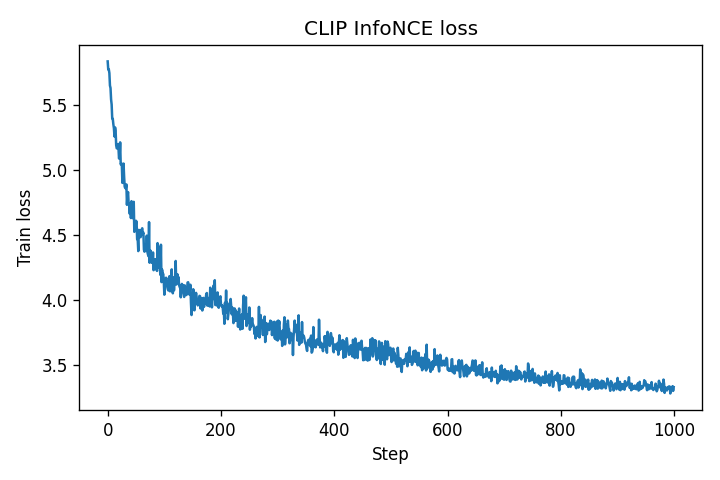
\includegraphics[width=0.82\linewidth]{figures/clip_eurosat/train_loss.png}
    \caption{CLIP pretraining loss on EuroSAT.}
    \label{fig:clip-train-loss}
\end{figure}

\begin{figure}[H]
    \centering
    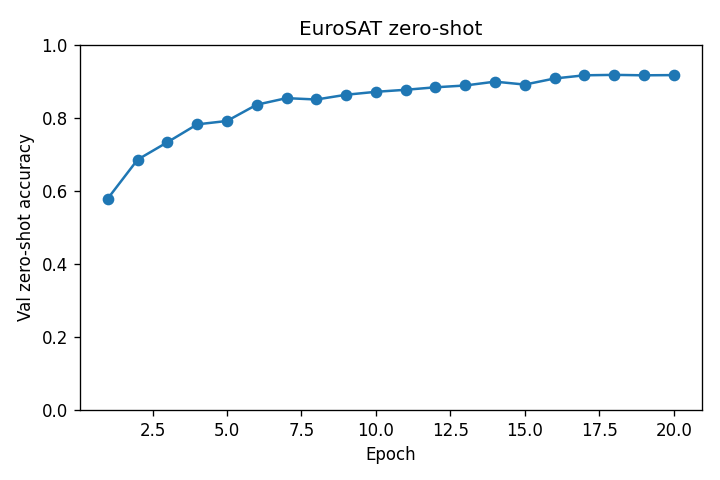
\includegraphics[width=0.82\linewidth]{figures/clip_eurosat/val_accuracy.png}
    \caption{Zero-shot validation accuracy during CLIP pretraining on EuroSAT.}
    \label{fig:clip-val-acc}
\end{figure}

The training loss decreases steadily from about $5.8$ at the start of training to about $3.3$ by the end, while zero-shot validation accuracy rises quickly in the first few epochs and then levels off near $92\%$. The best validation accuracy is $91.77\%$ at epoch 18, and the final epoch is essentially unchanged at $91.71\%$, so most of the validation improvement has saturated by the last few epochs. In contrast, the training loss continues to drift downward after the validation curve plateaus, suggesting the model is still fitting the contrastive training objective even though additional optimization is no longer translating into meaningful validation gains.

\subsection{Qualitative Zero-Shot Analysis}

\begin{figure}[H]
    \centering
    \fbox{\parbox[c][2.0in][c]{0.85\linewidth}{\centering \TODO{Insert 5 correct and 5 incorrect validation examples with predicted labels.}}}
    \caption{Qualitative zero-shot EuroSAT examples.}
    \label{fig:clip-qualitative}
\end{figure}

\begin{table}[H]
    \centering
    \begin{tabular}{llll}
        \toprule
        Example & Ground truth & Prediction & Top-3 predictions \\
        \midrule
        \TODO{1} & \TODO{} & \TODO{} & \TODO{} \\
        \TODO{2} & \TODO{} & \TODO{} & \TODO{} \\
        \TODO{3} & \TODO{} & \TODO{} & \TODO{} \\
        \TODO{4} & \TODO{} & \TODO{} & \TODO{} \\
        \TODO{5} & \TODO{} & \TODO{} & \TODO{} \\
        \bottomrule
    \end{tabular}
    \caption{Incorrect zero-shot EuroSAT examples and their top-3 predictions.}
    \label{tab:clip-mistakes}
\end{table}

\TODO{Write a 3--4 sentence discussion of whether the mistakes are reasonable and what they suggest about the learned embedding space.}

\section{LoRA Fine-Tuning}

\subsection{LoRA Linear Layer}

\begin{table}[H]
    \centering
    \begin{tabular}{ccc}
        \toprule
        Total parameters & Trainable parameters & Trainable ratio \\
        \midrule
        \TODO{} & \TODO{} & \TODO{} \\
        \bottomrule
    \end{tabular}
    \caption{Parameter counts for ViT with LoRA rank 8.}
    \label{tab:lora-params}
\end{table}

\subsection{Full Fine-Tuning vs. LoRA vs. Linear Probe}

\begin{table}[H]
    \centering
    \begin{tabular}{lcccc}
        \toprule
        Method & Test accuracy & Trainable parameters & Peak memory & Wall-clock time \\
        \midrule
        Linear probe & \TODO{} & \TODO{} & \TODO{} & \TODO{} \\
        LoRA rank 8 & \TODO{} & \TODO{} & \TODO{} & \TODO{} \\
        Full fine-tuning & \TODO{} & \TODO{} & \TODO{} & \TODO{} \\
        \bottomrule
    \end{tabular}
    \caption{RESISC45 adaptation comparison.}
    \label{tab:lora-compare}
\end{table}

\TODO{Write a 4--5 sentence discussion of the accuracy, memory, parameter, and time trade-offs.}

\subsection{LoRA Rank Sweep}

\begin{figure}[H]
    \centering
    \fbox{\parbox[c][1.7in][c]{0.8\linewidth}{\centering \TODO{Insert test accuracy vs. LoRA rank plot.}}}
    \caption{RESISC45 test accuracy as a function of LoRA rank.}
    \label{fig:lora-rank}
\end{figure}

\TODO{Write a 3--4 sentence discussion. Include the rank where returns diminish and how this compares to typical ranks such as 8 or 16.}

\section{Vision-Language Model}

\subsection{Vision-Language Projector}

\TODO{Write 1--2 sentences explaining why the projector uses a small MLP rather than a single linear layer.}

\subsection{Token Injection Strategies}

\begin{table}[H]
    \centering
    \begin{tabular}{lcccc}
        \toprule
        Injection strategy & Validation accuracy & Visual tokens & Peak memory & Time per step \\
        \midrule
        CLS-only prefix & \TODO{} & \TODO{} & \TODO{} & \TODO{} \\
        All-patches prefix & \TODO{} & \TODO{} & \TODO{} & \TODO{} \\
        Interleaved placeholder & \TODO{} & \TODO{} & \TODO{} & \TODO{} \\
        \bottomrule
    \end{tabular}
    \caption{CLEVR comparison of visual-token injection strategies.}
    \label{tab:vlm-injection}
\end{table}

\TODO{Write a 1-paragraph discussion of which strategy worked best and whether the extra cost was worth it. Connect this to the CLS-vs-patch pooling question.}

\subsection{Attention Masking}

\begin{figure}[H]
    \centering
    \begin{subfigure}{0.45\linewidth}
        \centering
        \fbox{\parbox[c][1.5in][c]{0.9\linewidth}{\centering \TODO{Draw 7x7 fully causal mask.}}}
        \caption{Fully causal mask}
    \end{subfigure}
    \hfill
    \begin{subfigure}{0.45\linewidth}
        \centering
        \fbox{\parbox[c][1.5in][c]{0.9\linewidth}{\centering \TODO{Draw 7x7 image-bidirectional mask.}}}
        \caption{Image-bidirectional mask}
    \end{subfigure}
    \caption{Attention masks for 4 visual tokens followed by 3 text tokens.}
    \label{fig:vlm-masks}
\end{figure}

\TODO{Write a 3--4 sentence discussion of which mask you expect to perform better and why.}

\begin{table}[H]
    \centering
    \begin{tabular}{lc}
        \toprule
        Mask mode & Validation accuracy \\
        \midrule
        Fully causal & \TODO{} \\
        Image-bidirectional & \TODO{} \\
        \bottomrule
    \end{tabular}
    \caption{CLEVR validation accuracy for attention-mask ablation.}
    \label{tab:vlm-masking}
\end{table}

\subsection{Freezing Strategies}

\begin{table}[H]
    \centering
    \begin{tabular}{lccc}
        \toprule
        Configuration & Validation accuracy & Trainable parameters & Peak memory \\
        \midrule
        Projector only & \TODO{} & \TODO{} & \TODO{} \\
        Projector + decoder LoRA & \TODO{} & \TODO{} & \TODO{} \\
        Projector + full decoder & \TODO{} & \TODO{} & \TODO{} \\
        Full fine-tuning & \TODO{} & \TODO{} & \TODO{} \\
        \bottomrule
    \end{tabular}
    \caption{CLEVR freezing-strategy comparison.}
    \label{tab:vlm-freezing}
\end{table}

\TODO{Write a 5--6 sentence discussion of the best accuracy/cost trade-off in the context of the two-stage VLM recipe.}

\subsection{Qualitative Evaluation}

\begin{table}[H]
    \centering
    \begin{tabular}{llll}
        \toprule
        Example & Question & Ground truth & Model generation \\
        \midrule
        \TODO{1} & \TODO{} & \TODO{} & \TODO{} \\
        \TODO{2} & \TODO{} & \TODO{} & \TODO{} \\
        \TODO{3} & \TODO{} & \TODO{} & \TODO{} \\
        \TODO{4} & \TODO{} & \TODO{} & \TODO{} \\
        \TODO{5} & \TODO{} & \TODO{} & \TODO{} \\
        \TODO{6} & \TODO{} & \TODO{} & \TODO{} \\
        \TODO{7} & \TODO{} & \TODO{} & \TODO{} \\
        \TODO{8} & \TODO{} & \TODO{} & \TODO{} \\
        \TODO{9} & \TODO{} & \TODO{} & \TODO{} \\
        \TODO{10} & \TODO{} & \TODO{} & \TODO{} \\
        \bottomrule
    \end{tabular}
    \caption{Qualitative CLEVR generations from the best VLM.}
    \label{tab:vlm-qualitative}
\end{table}

\TODO{Write a 4--5 sentence discussion of incorrect cases. Hypothesize encoder vs. decoder failures and propose an experiment to distinguish them.}

\section{Positional Encodings and RoPE}

\subsection{1D RoPE}

\begin{table}[H]
    \centering
    \begin{tabular}{cc}
        \toprule
        Quantity & Value \\
        \midrule
        Max norm difference after RoPE & \TODO{} \\
        \bottomrule
    \end{tabular}
    \caption{Manual norm-preservation check for \class{RoPE1D}.}
    \label{tab:rope-norm}
\end{table}

\subsection{Learned Positional Embeddings vs. 1D RoPE}

\begin{table}[H]
    \centering
    \begin{tabular}{lcc}
        \toprule
        Positional encoding & Train-size accuracy & 96x96 extrapolated accuracy \\
        \midrule
        Learned positional embeddings & \TODO{} & \TODO{} \\
        1D RoPE & \TODO{} & \TODO{} \\
        \bottomrule
    \end{tabular}
    \caption{EuroSAT learned-position vs. 1D RoPE comparison.}
    \label{tab:rope-1d}
\end{table}

\TODO{Write a 3--4 sentence discussion of extrapolation behavior and degradation at 96x96 resolution.}

\subsection{2D RoPE}

\begin{table}[H]
    \centering
    \begin{tabular}{lcc}
        \toprule
        Positional encoding & Train-size accuracy & 96x96 extrapolated accuracy \\
        \midrule
        1D RoPE & \TODO{} & \TODO{} \\
        2D RoPE & \TODO{} & \TODO{} \\
        \bottomrule
    \end{tabular}
    \caption{EuroSAT 1D RoPE vs. 2D RoPE comparison.}
    \label{tab:rope-2d}
\end{table}

\TODO{Write a 2--3 sentence discussion of whether 2D RoPE improved over 1D RoPE on EuroSAT.}

\subsection{Multimodal RoPE}

\paragraph{Naive 1D Position IDs.}
\TODO{Write one paragraph explaining what goes wrong with naive 1D position IDs when 64 patch tokens plus CLS are injected before a text prompt. Address decoder position ranges and loss of 2D image structure.}

\paragraph{First Text Position Under M-RoPE.}
\TODO{Write one paragraph explaining what position the first text token receives as a function of image grid size, and why this is sensible.}

\paragraph{Why Three Chunks.}
\TODO{Write one paragraph explaining why M-RoPE splits the head dimension into temporal, horizontal, and vertical chunks rather than using only x and y.}

\subsection{M-RoPE Bonus}

\begin{table}[H]
    \centering
    \begin{tabular}{lcc}
        \toprule
        Position assignment & Overall accuracy & Spatial-question accuracy \\
        \midrule
        Naive 1D position IDs & \TODO{} & \TODO{} \\
        M-RoPE-style position IDs & \TODO{} & \TODO{} \\
        \bottomrule
    \end{tabular}
    \caption{Optional M-RoPE bonus comparison on CLEVR.}
    \label{tab:mrope-bonus}
\end{table}

\TODO{If completing the bonus, write a 3--4 sentence discussion of whether M-RoPE improves overall and spatial-question accuracy. Otherwise, remove or mark this subsection as not attempted.}

\end{document}
